\documentclass[]{book}
\usepackage{lmodern}
\usepackage{amssymb,amsmath}
\usepackage{ifxetex,ifluatex}
\usepackage{fixltx2e} % provides \textsubscript
\ifnum 0\ifxetex 1\fi\ifluatex 1\fi=0 % if pdftex
  \usepackage[T1]{fontenc}
  \usepackage[utf8]{inputenc}
\else % if luatex or xelatex
  \ifxetex
    \usepackage{mathspec}
  \else
    \usepackage{fontspec}
  \fi
  \defaultfontfeatures{Ligatures=TeX,Scale=MatchLowercase}
\fi
% use upquote if available, for straight quotes in verbatim environments
\IfFileExists{upquote.sty}{\usepackage{upquote}}{}
% use microtype if available
\IfFileExists{microtype.sty}{%
\usepackage{microtype}
\UseMicrotypeSet[protrusion]{basicmath} % disable protrusion for tt fonts
}{}
\usepackage[margin=1in]{geometry}
\usepackage{hyperref}
\hypersetup{unicode=true,
            pdftitle={Statistics, R, and Music},
            pdfauthor={David John Baker},
            pdfborder={0 0 0},
            breaklinks=true}
\urlstyle{same}  % don't use monospace font for urls
\usepackage{natbib}
\bibliographystyle{apalike}
\usepackage{color}
\usepackage{fancyvrb}
\newcommand{\VerbBar}{|}
\newcommand{\VERB}{\Verb[commandchars=\\\{\}]}
\DefineVerbatimEnvironment{Highlighting}{Verbatim}{commandchars=\\\{\}}
% Add ',fontsize=\small' for more characters per line
\usepackage{framed}
\definecolor{shadecolor}{RGB}{248,248,248}
\newenvironment{Shaded}{\begin{snugshade}}{\end{snugshade}}
\newcommand{\KeywordTok}[1]{\textcolor[rgb]{0.13,0.29,0.53}{\textbf{{#1}}}}
\newcommand{\DataTypeTok}[1]{\textcolor[rgb]{0.13,0.29,0.53}{{#1}}}
\newcommand{\DecValTok}[1]{\textcolor[rgb]{0.00,0.00,0.81}{{#1}}}
\newcommand{\BaseNTok}[1]{\textcolor[rgb]{0.00,0.00,0.81}{{#1}}}
\newcommand{\FloatTok}[1]{\textcolor[rgb]{0.00,0.00,0.81}{{#1}}}
\newcommand{\ConstantTok}[1]{\textcolor[rgb]{0.00,0.00,0.00}{{#1}}}
\newcommand{\CharTok}[1]{\textcolor[rgb]{0.31,0.60,0.02}{{#1}}}
\newcommand{\SpecialCharTok}[1]{\textcolor[rgb]{0.00,0.00,0.00}{{#1}}}
\newcommand{\StringTok}[1]{\textcolor[rgb]{0.31,0.60,0.02}{{#1}}}
\newcommand{\VerbatimStringTok}[1]{\textcolor[rgb]{0.31,0.60,0.02}{{#1}}}
\newcommand{\SpecialStringTok}[1]{\textcolor[rgb]{0.31,0.60,0.02}{{#1}}}
\newcommand{\ImportTok}[1]{{#1}}
\newcommand{\CommentTok}[1]{\textcolor[rgb]{0.56,0.35,0.01}{\textit{{#1}}}}
\newcommand{\DocumentationTok}[1]{\textcolor[rgb]{0.56,0.35,0.01}{\textbf{\textit{{#1}}}}}
\newcommand{\AnnotationTok}[1]{\textcolor[rgb]{0.56,0.35,0.01}{\textbf{\textit{{#1}}}}}
\newcommand{\CommentVarTok}[1]{\textcolor[rgb]{0.56,0.35,0.01}{\textbf{\textit{{#1}}}}}
\newcommand{\OtherTok}[1]{\textcolor[rgb]{0.56,0.35,0.01}{{#1}}}
\newcommand{\FunctionTok}[1]{\textcolor[rgb]{0.00,0.00,0.00}{{#1}}}
\newcommand{\VariableTok}[1]{\textcolor[rgb]{0.00,0.00,0.00}{{#1}}}
\newcommand{\ControlFlowTok}[1]{\textcolor[rgb]{0.13,0.29,0.53}{\textbf{{#1}}}}
\newcommand{\OperatorTok}[1]{\textcolor[rgb]{0.81,0.36,0.00}{\textbf{{#1}}}}
\newcommand{\BuiltInTok}[1]{{#1}}
\newcommand{\ExtensionTok}[1]{{#1}}
\newcommand{\PreprocessorTok}[1]{\textcolor[rgb]{0.56,0.35,0.01}{\textit{{#1}}}}
\newcommand{\AttributeTok}[1]{\textcolor[rgb]{0.77,0.63,0.00}{{#1}}}
\newcommand{\RegionMarkerTok}[1]{{#1}}
\newcommand{\InformationTok}[1]{\textcolor[rgb]{0.56,0.35,0.01}{\textbf{\textit{{#1}}}}}
\newcommand{\WarningTok}[1]{\textcolor[rgb]{0.56,0.35,0.01}{\textbf{\textit{{#1}}}}}
\newcommand{\AlertTok}[1]{\textcolor[rgb]{0.94,0.16,0.16}{{#1}}}
\newcommand{\ErrorTok}[1]{\textcolor[rgb]{0.64,0.00,0.00}{\textbf{{#1}}}}
\newcommand{\NormalTok}[1]{{#1}}
\usepackage{longtable,booktabs}
\usepackage{graphicx,grffile}
\makeatletter
\def\maxwidth{\ifdim\Gin@nat@width>\linewidth\linewidth\else\Gin@nat@width\fi}
\def\maxheight{\ifdim\Gin@nat@height>\textheight\textheight\else\Gin@nat@height\fi}
\makeatother
% Scale images if necessary, so that they will not overflow the page
% margins by default, and it is still possible to overwrite the defaults
% using explicit options in \includegraphics[width, height, ...]{}
\setkeys{Gin}{width=\maxwidth,height=\maxheight,keepaspectratio}
\IfFileExists{parskip.sty}{%
\usepackage{parskip}
}{% else
\setlength{\parindent}{0pt}
\setlength{\parskip}{6pt plus 2pt minus 1pt}
}
\setlength{\emergencystretch}{3em}  % prevent overfull lines
\providecommand{\tightlist}{%
  \setlength{\itemsep}{0pt}\setlength{\parskip}{0pt}}
\setcounter{secnumdepth}{5}
% Redefines (sub)paragraphs to behave more like sections
\ifx\paragraph\undefined\else
\let\oldparagraph\paragraph
\renewcommand{\paragraph}[1]{\oldparagraph{#1}\mbox{}}
\fi
\ifx\subparagraph\undefined\else
\let\oldsubparagraph\subparagraph
\renewcommand{\subparagraph}[1]{\oldsubparagraph{#1}\mbox{}}
\fi

%%% Use protect on footnotes to avoid problems with footnotes in titles
\let\rmarkdownfootnote\footnote%
\def\footnote{\protect\rmarkdownfootnote}

%%% Change title format to be more compact
\usepackage{titling}

% Create subtitle command for use in maketitle
\newcommand{\subtitle}[1]{
  \posttitle{
    \begin{center}\large#1\end{center}
    }
}

\setlength{\droptitle}{-2em}
  \title{Statistics, R, and Music}
  \pretitle{\vspace{\droptitle}\centering\huge}
  \posttitle{\par}
  \author{David John Baker}
  \preauthor{\centering\large\emph}
  \postauthor{\par}
  \predate{\centering\large\emph}
  \postdate{\par}
  \date{2017-09-05}

\usepackage{booktabs}

\usepackage{amsthm}
\newtheorem{theorem}{Theorem}[chapter]
\newtheorem{lemma}{Lemma}[chapter]
\theoremstyle{definition}
\newtheorem{definition}{Definition}[chapter]
\newtheorem{corollary}{Corollary}[chapter]
\newtheorem{proposition}{Proposition}[chapter]
\theoremstyle{definition}
\newtheorem{example}{Example}[chapter]
\theoremstyle{definition}
\newtheorem{exercise}{Exercise}[chapter]
\theoremstyle{remark}
\newtheorem*{remark}{Remark}
\newtheorem*{solution}{Solution}
\begin{document}
\maketitle

{
\setcounter{tocdepth}{1}
\tableofcontents
}
\chapter{Introduction to Statistics}\label{introduction-to-statistics}

What this book will assume

\begin{itemize}
\tightlist
\item
  Basic knowledge of math
\item
  Basic computer literacy
\item
  Include chapter on levels of measuremet? Aka Chapter 1-4 Cohen?
\item
  Ability to look for answers self, working with R you need to be able
  to troubleshoot
\end{itemize}

What book plans to accomplish

\begin{itemize}
\tightlist
\item
  Grounding in basic NHST statistics
\item
  Teach basic calculations by hand
\item
  Working knowldge of R for all tests
\item
  Manipulating data in R
\item
  Basic visualization of data in R
\item
  Guide to finding similar values from SPSS
\end{itemize}

This is a \emph{sample} book written in \textbf{Markdown}. You can use
anything that Pandoc's Markdown supports, e.g., a math equation
\(a^2 + b^2 = c^2\).

For now, you have to install the development versions of
\textbf{bookdown} from Github:

\begin{Shaded}
\begin{Highlighting}[]
\NormalTok{devtools::}\KeywordTok{install_github}\NormalTok{(}\StringTok{"rstudio/bookdown"}\NormalTok{)}
\end{Highlighting}
\end{Shaded}

Remember each Rmd file contains one and only one chapter, and a chapter
is defined by the first-level heading \texttt{\#}.

To compile this example to PDF, you need to install XeLaTeX.

\chapter{Sampling Distributions and T-Tests}\label{intro}

You can label chapter and section titles using \texttt{\{\#label\}}
after them, e.g., we can reference Chapter \ref{intro}. If you do not
manually label them, there will be automatic labels anyway, e.g.,
Chapter \ref{methods}.

Figures and tables with captions will be placed in \texttt{figure} and
\texttt{table} environments, respectively.

\begin{Shaded}
\begin{Highlighting}[]
\KeywordTok{par}\NormalTok{(}\DataTypeTok{mar =} \KeywordTok{c}\NormalTok{(}\DecValTok{4}\NormalTok{, }\DecValTok{4}\NormalTok{, .}\DecValTok{1}\NormalTok{, .}\DecValTok{1}\NormalTok{))}
\KeywordTok{plot}\NormalTok{(pressure, }\DataTypeTok{type =} \StringTok{'b'}\NormalTok{, }\DataTypeTok{pch =} \DecValTok{19}\NormalTok{)}
\end{Highlighting}
\end{Shaded}

\begin{figure}

{\centering 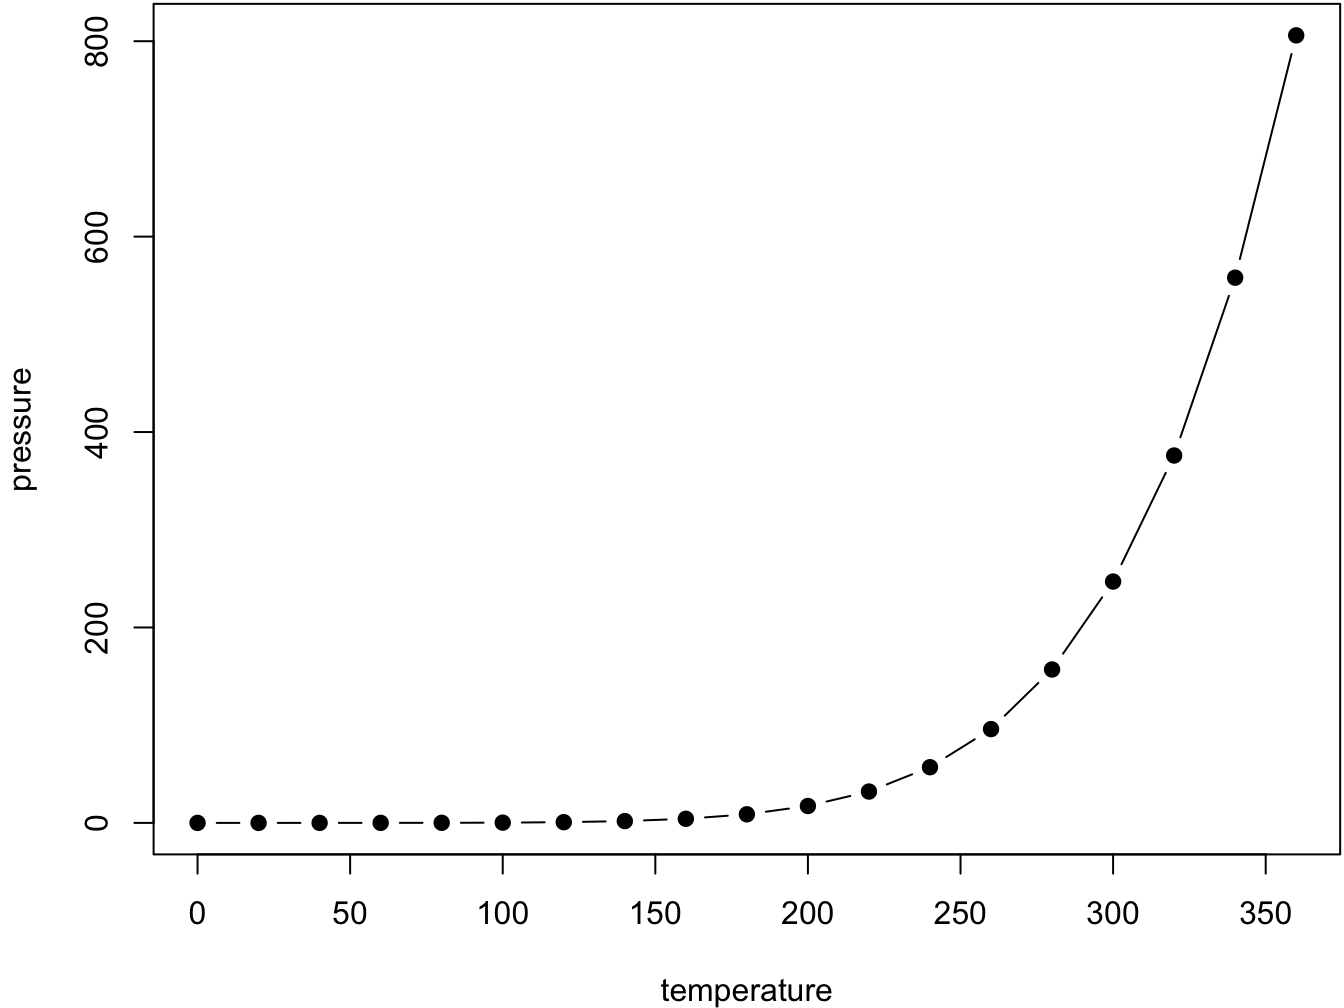
\includegraphics[width=0.8\linewidth]{bookdown-demo_files/figure-latex/nice-fig-1} 

}

\caption{Here is a nice figure!}\label{fig:nice-fig}
\end{figure}

Reference a figure by its code chunk label with the \texttt{fig:}
prefix, e.g., see Figure \ref{fig:nice-fig}. Similarly, you can
reference tables generated from \texttt{knitr::kable()}, e.g., see Table
\ref{tab:nice-tab}.

\begin{Shaded}
\begin{Highlighting}[]
\NormalTok{knitr::}\KeywordTok{kable}\NormalTok{(}
  \KeywordTok{head}\NormalTok{(iris, }\DecValTok{20}\NormalTok{), }\DataTypeTok{caption =} \StringTok{'Here is a nice table!'}\NormalTok{,}
  \DataTypeTok{booktabs =} \OtherTok{TRUE}
\NormalTok{)}
\end{Highlighting}
\end{Shaded}

\begin{table}

\caption{\label{tab:nice-tab}Here is a nice table!}
\centering
\begin{tabular}[t]{rrrrl}
\toprule
Sepal.Length & Sepal.Width & Petal.Length & Petal.Width & Species\\
\midrule
5.1 & 3.5 & 1.4 & 0.2 & setosa\\
4.9 & 3.0 & 1.4 & 0.2 & setosa\\
4.7 & 3.2 & 1.3 & 0.2 & setosa\\
4.6 & 3.1 & 1.5 & 0.2 & setosa\\
5.0 & 3.6 & 1.4 & 0.2 & setosa\\
\addlinespace
5.4 & 3.9 & 1.7 & 0.4 & setosa\\
4.6 & 3.4 & 1.4 & 0.3 & setosa\\
5.0 & 3.4 & 1.5 & 0.2 & setosa\\
4.4 & 2.9 & 1.4 & 0.2 & setosa\\
4.9 & 3.1 & 1.5 & 0.1 & setosa\\
\addlinespace
5.4 & 3.7 & 1.5 & 0.2 & setosa\\
4.8 & 3.4 & 1.6 & 0.2 & setosa\\
4.8 & 3.0 & 1.4 & 0.1 & setosa\\
4.3 & 3.0 & 1.1 & 0.1 & setosa\\
5.8 & 4.0 & 1.2 & 0.2 & setosa\\
\addlinespace
5.7 & 4.4 & 1.5 & 0.4 & setosa\\
5.4 & 3.9 & 1.3 & 0.4 & setosa\\
5.1 & 3.5 & 1.4 & 0.3 & setosa\\
5.7 & 3.8 & 1.7 & 0.3 & setosa\\
5.1 & 3.8 & 1.5 & 0.3 & setosa\\
\bottomrule
\end{tabular}
\end{table}

You can write citations, too. For example, we are using the
\textbf{bookdown} package \citep{R-bookdown} in this sample book, which
was built on top of R Markdown and \textbf{knitr} \citep{xie2015}.

\chapter{Confidence Intervals and
Power}\label{confidence-intervals-and-power}

Class notes from September 5th, 2017

\section{Confidence Interval
Estimation}\label{confidence-interval-estimation}

Confidence intervals are a way to get at a range of likely values for an
estimate. It's an inferrential way of thinking about values from your
sample. It differs from things like the mean, median, and mode in that
those are point esitmates and a CI is a range.

We know that over repeated sampling, the CI represents the percentage of
sugt intervals that contain the population mean. Just like a p value,
you can set the CI to any percentage you want. So just like you can
think of a distribution of sample means as a way of describing your
parameters, you can also do this with CIs.

A CI gives you an educated guess of identifying the population mean than
just knowing one number, which would be the mean itself. Keep in mind
for all of this we are operating on the sampling distribution
informaiton. Just like the set of t distributions are a set of sampling
distributions, CIs are computed from the sampling distributions.

There is a relationship between CIs and p values because at their core
is the sampling distribution. They are not the same thing, but they
represent information coming from the sampling distribution.

Take a look at the image below. We see here in an image taken from THIS
that we can see what a confidence interval is. Image you take a sample
from known populaiton paramters. We tell it we want a certain N, mu, and
standard deviation. What it then does is construct a CI around that
mean. We have a certain amount of information that comes from our
sample. Our CI is a symmetrical range that gives you a sense of the
possibilites of where the populatin mean might be.

IMAGE WITH ONE

It's not a probability of the mean being in that CI! A CI represents the
percentage of intervals that capture the population mean. This only
makes sense if you think about repeated sampling over many experiments.
You then calculate the number of intervals that contain the actual
population mean.

IMAGE BLACK RED

IMAGE WITH ALL OF THEM.

So now below you can see 25 samples. You can start to see teh sampling
distribution get created at the bottom They start to form a normal
curve. Notice that every sample mean has a symmetrical intervals. Note
that there are 2 sample means and their CI, the entire interval does not
have the population mean. But for all of the other ones, they do have
the population mean. So 23/25 is 92\%, but as we add more in we would
eventually add more and approach 95\%. Any one of these intervals gives
you an estimate of the populatino mean. That does not mean its 95\%
likely to be right. It's that in repeated samples 95\% of the samples
will fall in that range. What we have now is a range of values that
might hold the mean. 95\% of these will have mean in the long run.

Note that with the sampling distribution at the bottom, we are still
using information. We still use mean, the standard error. We still know
the degrees of freedom.

Note that this is just a visualzation. Note some of the intervals are
wider, some are shoter. This is because your samples SD is goign to hop
around. The sample's CI takes into account the standard error.

We can see now see the difference in means between two sample means. We
now plot the difference from TTESTFROM EARLIER. We subtract the two
means and can see in the long run, we had a population mean of 10. But
if you look at it, note that the populations hop around. Not only that,
but they all have CIs.

With this image, if the Null was true, we would get means around 0. Note
that a lot of these random samples from a known population that is not
the null, over HALF of them make it look like the null could be a
reasonable guess. Just like a NHT, sometimes you are going to get a high
P value even though we know the Null is false. Why might this happen?
Well it might just be that we need to figure out how to set up.

\section{Example}\label{example}

Let's return to the example that we are looking at SAT scores with a
population mean of 455. We then calculate the 95\% confidence interval.
What it's trying to do is capture the inside part. Note your CI is not
exactly the mean and the cut off boundary, your mean changes. This is
just a reminder we use the sampling distribution interval.

SAMPLING DISTRIBUTION SAT IMAGE

\section{Computation of Confidece
Interval}\label{computation-of-confidece-interval}

Confidence interval for a single sample mean.

\[\bar{X} ± (t_{cv}s_{\bar{X}})\]

Note all we are doing is rearranging the t formulat. We multiply both
times by the standard error. It's not your actual t value, it's the
critical value of t. When you have two samples, you just rearrange the
values.

\[(\bar{X_{1}}-\bar{X_{1}}) ± (t_{cv})(s_{\bar{X_{1}}-\bar{X_{1}}})\]

Remember we are assuming we are constructing this from the sample means.
Let's return to our example from last chapter. We know the specific
numbers from each of our sample means.

PUT IN NUMBERS HERE IN TABLE.

Let's find out what happens when we look at each on interms of its own
mean and a difference. We don't know the population mean, so we go with
the sample mean.

\(t_{cv,df = 149,\alpha=.05,two tailed}= ± 1.97\)

CALCULATION HERE FOR SPRING AND FALL CLASS! \emph{NOte they are almost
identical}

SEE IF YOU CAN COLOR CODE THIS!!!

Note that at this point we are not comparing them against each other.
This says beyond just knowing the mean, says interval. This does not
mean the population mean is 95\% likely to be in that interval. It is if
I did this over and over, that 95\% of those intervals will hold the
sample mean.

The reasons we know this is because it's better than using the mean
alone. Report the CI like it is a descritive statistc. Though note that
this comes from the sampling distribution, which comes from an
infferential.

\chapter{Methods}\label{methods}

We describe our methods in this chapter.

\chapter{Applications}\label{applications}

Some \emph{significant} applications are demonstrated in this chapter.

\section{Example one}\label{example-one}

\section{Example two}\label{example-two}

\chapter{Final Words}\label{final-words}

We have finished a nice book.

\bibliography{packages.bib,book.bib}


\end{document}
